
\section{Cellular automata}
In LGCA we have different restrictions which simplifies our computations and decrease the computation costs, in comparison to MD. For example molecule-to-molecule forces are replaced with rigid body collisions, and during one time step, particles can travel only along one edge.  The velocities are discretized too, what implies that all particles have the same energy and at the end of a time step particles can reside only at vertices.
The first lattice-gas cellular automata (LGCA) was proposed in 1973 by Hardy, de Pazzis and Pomeau [3]. It is named HPP and is a CA model over square lattice. HPP does not lead to Navier-Stokes equations, because of insufficient degree of rotational symmetry of the lattice. But still it worth of discussion, and we will do it later on.

Frish-Hasslacher-Pomeau is the model of LGCA (see Fig. 1), which lead to Navier-Stokes equations, because of it's symmetry. For example Frish-Hasslacher-Pomeau automata has following prescriptions [2]:

\begin{itemize}
\item All particles have the same mass m=1.
\item Particles can move only along one of the six directions defined by the discrete displacements $c_{i}$.
\item In a time-cycle (made one for convenience) the particles hop to the neares neighbor pointed by the corresponding discrete vector $c_{i}$. Both longer and shorter jumps are forbidden which means all lattice particles have the same energy.
\item No two particles sitting on the same site can move along the same direction $c_{i}$ (exclusion principle).
\end{itemize}

\begin{figure}[H]
  \centering
  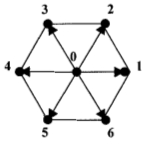
\includegraphics[width=0.1\textwidth]{img/fig1.png}
  \caption{The FHP hexagonal lattice [2].}
\end{figure}

In LGCA we have such basic mechanisms:

\begin{itemize}
\item Free-streaming: $ n_i^{in}(\vec{r}+\vec{c}_{i}\Delta t, t+\Delta t) = n_i^{out}(\vec{r}, t) $
\item Collision: $ n_i^{out}(\vec{r}, t) = n_i^{in}(\vec{r}, t) + \Omega(n_i^{in}(\vec{r}, t)) $.
\end{itemize}
Where $\Omega$ is a collision operator.

Free-streaming is a simple transfer of particles according of their discrete velocities.

When two particles meet each other on the site they interact and exchange their momenta following the discretization rules of the lattice. Such exchange is called collision. In HPP only two particles can collide, that is why the collision in HPP is deterministic(see Fig. 2 (a)).

If we will consider the collision of two particles in FHP, then we will have non-deterministic outcome(see Fig. 2 (b)).


\begin{figure}[H]
  \centering
  \begin{subfigure}[h]{0.5\textwidth}
    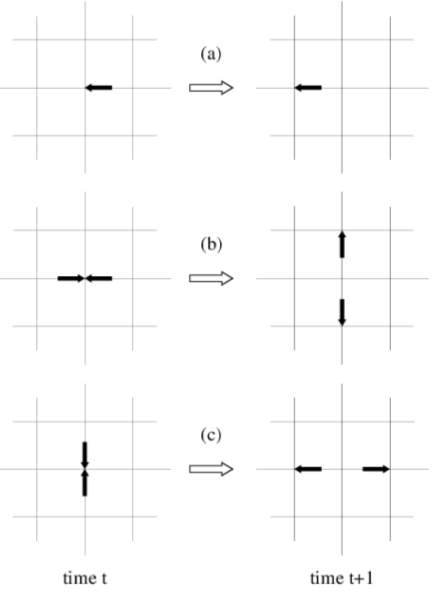
\includegraphics[width=\textwidth]{img/fig4.png}
    \caption{HHP streaming(a)/collision(b,c) [6].}
  \end{subfigure}
  \begin{subfigure}[h]{0.3\textwidth}
    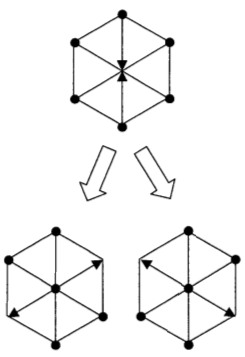
\includegraphics[width=\textwidth]{img/fig5.png}
    \caption{FHP collision [2].}
  \end{subfigure}
  \caption{Collision of two particles / streaming.}
\end{figure}

Albeit all restrictions this collision shares two crucial features such as conversation of particle number and conversation of the total momentum.

\begin{itemize}
\item conserve mass (number of particles): $ \sum_i n_i^{in} = \sum_i n_i^{out} $
\item conserve momentum: $ \sum_i n_i^{in} \vec{c}_{ia} = \sum_i n_i^{out} \vec{c}_{ia} $
\end{itemize}

The exclusion principle is kept too. There are no two particles with the same position and velocity at the same time.

One of the biggest advantages of LGCA is it's easy implementation, and  the easiness of it's parallelization, because of locality behaviour of the collision operator.

But the discretization works not always. For Macro-view such discretization is not a big problem, because we always discretize, but for Micro-view such restrictions can bring to huge inconsistency and very poor precision. Restriction in velocity direction and magnitude cannot describe model on microscopic level. In LGCA includes state of particle where the velocity is equal to zero(stationary particles), but in real word of microscopic level there can not exist such particles. There several main drawbacks of LGCA, but the most important one is statistical noise.

Lattice-Boltzmann approach was created as a respond on the main problems of LGCA, using an statistical averaging procedure.
